\subsection{Panel fizjoterapeuty}\label{subsec:panel-fizjoterapeuty}

{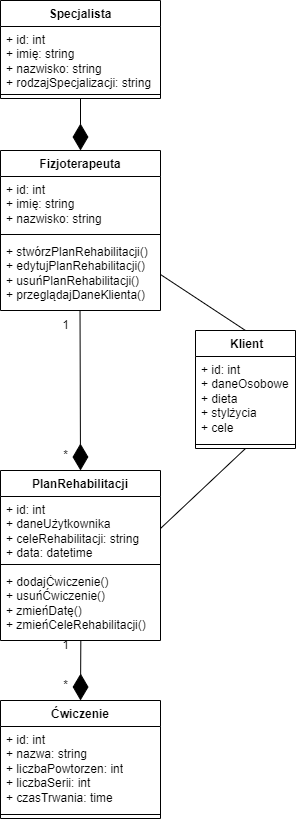
\includegraphics{../diagrams/use_cases/fizjoterapeuta}}

\begin{enumerate}
\setcounter{enumi}{3}
\tightlist
\item
  {Stwórz plan rehabilitacji}
\end{enumerate}


{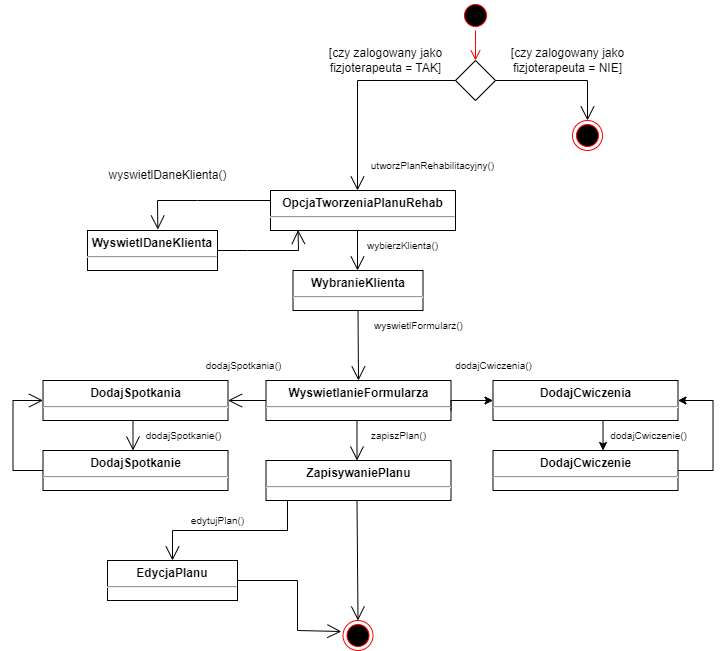
\includegraphics{../diagrams/state/tworzenie_planu_rehabilitacyjnego}}

{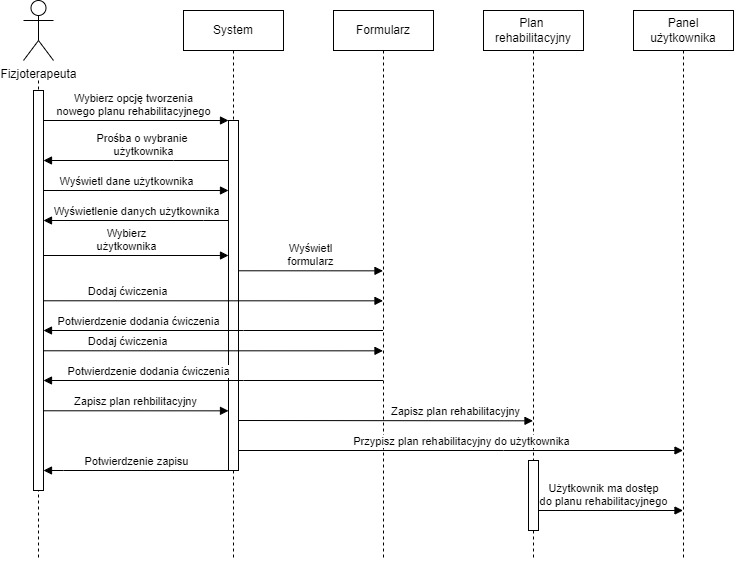
\includegraphics{../diagrams/sequence/tworzenie_planu_rehabilitacyjnego_sekwencja}}

{~~~~~~~~}{Aktorzy biorący udział: Fizjoterapeuta}

{~~~~~~~~Cel przypadku: Utworzenie planu rehabilitacji dla klienta}

{~~~~~~~~Warunki początkowe: Użytkownik jest zalogowany w systemie i ma
dostęp do panelu fizjoterapeuty.}

{~~~~~~~~Warunki końcowe: Utworzony został nowy plan rehabilitacji
dostępny dla klienta.}

{~~~~~~~~Główny ciąg zdarzeń:}

\begin{enumerate}
\tightlist
\item
  {Użytkownik wybiera klienta docelowego.}
\item
  {Fizjoterapeuta ~przegląda dane klienta dotyczące jego aktualnej
  diety, stylu życia oraz jego aktualnego planu treningowego.}
\item
  {Użytkownik tworzy nowy plan rehabilitacji dodając odpowiednie
  ćwiczenia oraz terminy na masaże/konsultacje.}
\item
  {Fizjoterapeuta zapisuje plan w systemie.}
\end{enumerate}

{~~~~~~~~Alternatywny ciąg zdarzeń:}

{~~~~~~~~1a. Użytkownik nie posiada uprawnień fizjoterapeuty.}

\begin{itemize}
\tightlist
\item
  {System wyświetla komunikat o braku uprawnień.}
\end{itemize}

{~~~~~~~~1b. Użytkownik nie istnieje w systemie.}

\begin{itemize}
\tightlist
\item
  {System wyświetla komunikat o błędzie i prosi o podanie poprawnych
  danych.}
\end{itemize}

{~~~~~~~~2a. Fizjoterapeuta przegląda aktualny plan rehabilitacji.}

{~~~~~~~~3a. Fizjoterapeuta dodaje nowy plan rehabilitacji, dodaje
komentarze, uwagi.}

{}

\begin{enumerate}
\setcounter{enumi}{4}
\tightlist
\item
  {Edytuj plan rehabilitacji}
\end{enumerate}

{~~~~~~~~}{Aktorzy biorący udział: Fizjoterapeuta}

{~~~~~~~~Cel przypadku: Modyfikacja istniejącego już planu
rehabilitacji}

{~~~~~~~~Warunki początkowe: Użytkownik jest zalogowany w systemie i ma
dostęp do panelu fizjoterapeuty.}

{Warunki końcowe: Zmodyfikowany został plan rehabilitacji danego
klienta}

{Główny ciąg zdarzeń:}

\begin{enumerate}
\tightlist
\item
  {Użytkownik wybiera klienta docelowego.}
\item
  {Fizjoterapeuta przegląda dane klienta, jego plan rehabilitacji.}
\item
  {Użytkownik modyfikuje plan rehabilitacji, dodając komentarze, nowe
  ćwiczenia, modyfikując lub usuwając stare.}
\item
  {Fizjoterapeuta zapisuje plan w systemie}
\end{enumerate}

{~~~~~~~~Alternatywny ciąg zdarzeń:}

{1a. Użytkownik nie posiada uprawnień fizjoterapeuty.}

\begin{itemize}
\tightlist
\item
  {System wyświetla komunikat o braku uprawnień.}
\end{itemize}

{~~~~~~~~1b. Użytkownik nie istnieje w systemie.}

\begin{itemize}
\tightlist
\item
  {System wyświetla komunikat o błędzie i prosi o podanie poprawnych
  danych.}
\end{itemize}

{2a. Brak planu rehabilitacji:}

\begin{itemize}
\tightlist
\item
  {System informuje użytkownika o braku planu rehabilitacji, daje opcję
  przejścia do panelu tworzenia nowego planu rehabilitacji.}
\end{itemize}

{}

{}

{}

{}

\begin{enumerate}
\setcounter{enumi}{5}
\tightlist
\item
  {Usuń plan rehabilitacji}{\hfill\break
  Aktorzy biorący udział: Fizjoterapeuta}
\end{enumerate}

{~~~~~~~~Cel przypadku: Usunięcie planu rehabilitacji klienta.}

{~~~~~~~~Warunki początkowe: ~Użytkownik jest zalogowany w systemie i ma
dostęp do panelu fizjoterapeuty.}

{~~~~~~~~Warunki końcowe: Plan rehabilitacji został usunięty z profilu
użytkownika.}

{~~~~~~~~Główny ciąg zdarzeń:}

\begin{enumerate}
\tightlist
\item
  {Użytkownik wybiera klienta docelowego.}
\item
  {System wyświetla aktualny plan rehabilitacji danego użytkownika.}
\item
  {Po potwierdzeniu, system usuwa plan rehabilitacji.}
\item
  {System wyświetla potwierdzenie usunięcia planu rehabilitacji.}
\end{enumerate}

{~~~~~~~~Alternatywny ciąg zdarzeń:}

{~~~~~~~~1a. Użytkownik nie posiada uprawnień fizjoterapeuty.}

\begin{itemize}
\tightlist
\item
  {System wyświetla komunikat o braku uprawnień.}
\end{itemize}

{~~~~~~~~1b. Użytkownik nie istnieje w systemie.}

\begin{itemize}
\tightlist
\item
  {System wyświetla komunikat o błędzie i prosi o podanie poprawnych
  danych.}
\end{itemize}

{~~~~~~~~2a. Brak planu rehabilitacji:}

\begin{itemize}
\tightlist
\item
  {System informuje użytkownika o braku planu rehabilitacji}
\end{itemize}

{3a. Fizjoterapeuta nie potwierdza usunięcia planu
rehabilitacji, skutkuje to informacją systemu.}